% THIS DOCUMENT IS FOLLOWS THE VOLERE TEMPLATE BY Suzanne Robertson and James Robertson
% ONLY THE SECTION HEADINGS ARE PROVIDED
%
% Initial draft from https://github.com/Dieblich/volere
%
% Risks are removed because they are covered by the Hazard Analysis
\documentclass[12pt]{article}

\usepackage{booktabs}
\usepackage{tabularx}
\usepackage{hyperref}
\hypersetup{
    bookmarks=true,         % show bookmarks bar?
      colorlinks=true,      % false: boxed links; true: colored links
    linkcolor=red,          % color of internal links (change box color with linkbordercolor)
    citecolor=green,        % color of links to bibliography
    filecolor=magenta,      % color of file links
    urlcolor=cyan           % color of external links
}
\usepackage{amsmath, mathtools}
\usepackage{amsfonts}
\usepackage{amssymb}
\usepackage{graphicx}
\usepackage{colortbl}
\usepackage{xr}
\usepackage{longtable}
\usepackage{xfrac}
\usepackage{float}
\usepackage{siunitx}
\usepackage{caption}
\usepackage{pdflscape}
\usepackage{afterpage}
\usepackage{float}
\usepackage{fullpage}
\usepackage[round]{natbib}

\newcommand{\lips}{\textit{Insert your content here.}}

\input{../Comments}
\input{../Common}

% For easy change of table widths
\newcommand{\colZwidth}{1.0\textwidth}
\newcommand{\colAwidth}{0.13\textwidth}
\newcommand{\colBwidth}{0.82\textwidth}
\newcommand{\colCwidth}{0.1\textwidth}
\newcommand{\colDwidth}{0.05\textwidth}
\newcommand{\colEwidth}{0.8\textwidth}
\newcommand{\colFwidth}{0.17\textwidth}
\newcommand{\colGwidth}{0.5\textwidth}
\newcommand{\colHwidth}{0.28\textwidth}

% Used so that cross-references have a meaningful prefix
\newcounter{defnum} %Definition Number
\newcommand{\dthedefnum}{GD\thedefnum}
\newcommand{\dref}[1]{GD\ref{#1}}
\newcounter{datadefnum} %Datadefinition Number
\newcommand{\ddthedatadefnum}{DD\thedatadefnum}
\newcommand{\ddref}[1]{DD\ref{#1}}
\newcounter{theorynum} %Theory Number
\newcommand{\tthetheorynum}{TM\thetheorynum}
\newcommand{\tref}[1]{TM\ref{#1}}
\newcounter{tablenum} %Table Number
\newcommand{\tbthetablenum}{TB\thetablenum}
\newcommand{\tbref}[1]{TB\ref{#1}}
\newcounter{assumpnum} %Assumption Number
\newcommand{\atheassumpnum}{A\theassumpnum}
\newcommand{\aref}[1]{A\ref{#1}}
\newcounter{goalnum} %Goal Number
\newcommand{\gthegoalnum}{GS\thegoalnum}
\newcommand{\gsref}[1]{GS\ref{#1}}
\newcounter{stretchgoalnum} %Stretch Goal Number
\newcommand{\sgthestretchgoalnum}{STG\thestretchgoalnum}
\newcommand{\sgref}[1]{STG\ref{#1}}
\newcounter{instnum} %Instance Number
\newcommand{\itheinstnum}{IM\theinstnum}
\newcommand{\iref}[1]{IM\ref{#1}}
\newcounter{reqnum} %Requirement Number
\newcommand{\rthereqnum}{R\thereqnum}
\newcommand{\rref}[1]{R\ref{#1}}
\newcounter{nfrnum} %NFR Number
\newcommand{\rthenfrnum}{NFR\thenfrnum}
\newcommand{\nfrref}[1]{NFR\ref{#1}}
\newcounter{lcnum} %Likely change number
\newcommand{\lthelcnum}{LC\thelcnum}
\newcommand{\lcref}[1]{LC\ref{#1}}
\newcounter{ulcnum} %Unlikely change number
\newcommand{\ltheulcnum}{ULC\theulcnum}
\newcommand{\ulcref}[1]{ULC\ref{#1}}

\begin{document}

\title{Software Requirements Specification for \progname: RapidCare} 
\author{\authname}
\date{\today}
	
\maketitle

~\newpage

\pagenumbering{roman}

\tableofcontents

~\newpage

\section*{Revision History}

\begin{tabularx}{\textwidth}{p{3cm}p{2cm}X}
\toprule {\textbf{Date}} & {\textbf{Version}} & {\textbf{Notes}}\\
\midrule
12-10-2025 & 1.0 & Rev 0\\
06-01-2025 & 1.1 & Pranav Updated: TA feedback parts (Removed implementation details, fixed wordings, Traceability Matrix)\\
19-03-2025 & 1.2 & Template Update \\
\bottomrule
\end{tabularx}

~\\

~\newpage

\section{Introduction}

\subsection{Purpose of Document} \label{sec_PurposeOfDocument}
The purpose of this document is to provide a comprehensive description of the requirements for a software application that aims to streamline the healthcare documentation process aimed to be run as a web application. This document will be used in as a contract in a sense between the team and the client who intends to use this application. This document will allow for an in-depth description of the software's functionality, performance, and other non-functional requirements. Additionally, it will outline common use-cases under which the software will be used. This will in turn provide a direction to the developers such that they will be empowered to creating the right product as this document will contain various stakeholders' requirements. Along with development direction, this document will be a direct reference for all of the stakeholders to understand the product's scope, functionality, and limitations.

\subsection{Characteristics of Intended Reader} \label{sec_IntendedReader} 

The intended readers of this SRS document include project managers, software developers, testing engineers, and stakeholders directly involved in the design and implementation of the software system. Project managers and testing engineers would be directly involved in the development and testing process. They would generally have an education in computer science along with experience in software design, web or mobile development, and software testing. Project managers generally have experience in managing software projects and knowledge of software development processes. Stakeholders like doctors and nursing staff would have domain knowledge and could provide insights to understand the clinical workflow and documentation process. 


\section{Purpose of the Project}

\subsection{User Business}

\subsection{Goals of the Project}
% Gurleen copy from PS
% not completed

\section{Stakeholders}

\subsection{Client}
The primary client for this project are healthcare institutions such as hospitals and clinics. These institutions will benefit from the project as it will help in streamlining the documentation process, reducing administrative overhead, and enhancing the quality of patient care.

\subsection{Customer}
The primary customer of the project are healthcare professionals, specifically those involved in patient documentation, including doctors, nurses, and other clinical administrative staff. The project will provide a user-friendly interface that allows for efficient data entry and retrieval, as well as accurate transcription of patient interactions. The ystem will minimize the time spent on documentation, allowing them to focus more on patient care.

\subsection{Other Stakeholders}
\begin{itemize}
  \item \textbf{Society:} Society is a major stakeholder in this project. The healthcare institutions such as hospitals and clinics are a part of users group within the society that will be benefitted with improved efficiency. Additionally, they will be able to manage their staff better which in turn help in managing cost. Moreover, this project will help patients to get improved access to healthcare which will benenfit the society. 
  \item \textbf{Regulatory Bodies:} These are  the organizations that set standards for healthcare technology and data protection. They are concerned with compliance to regulations such as PIPEDA and other relevant laws.
\end{itemize}

\subsection{Hands-On Users of the Project}
\begin{itemize}
  \item\textbf{Healthcare Professionals:} These include the hospital staff such as Doctors, nurses etc, who will use the system.
  \item\textbf{Healthcare Network Employees:} These are the people employed in the organization who keeps records of all hospital facilities, their staff members and authenticates the healthcare professionals so that they are able to use the system. 
\end{itemize}

\subsection{Personas}
\begin{itemize}
    \item \textbf{Healthcare Professional: Dr. Virat} - Dr. Virat works in the emergency department at Brampton Hospital. He frequently uses EHR systems to document clinical notes and manage patient records. However, he feels that most of his time is spent recording notes. He wishes for a system that could speed up this process and allow him to focus more on direct patient care and serve more patients throughout the day.
    \item \textbf{Nurse: Anushka} - Anushka is a registered nurse who relies on the system to access patient information quickly and update records during patient triage. She often feel streesed due to increased patient volume and long hours of shift due to inefficent staff maangmement at her hospital.
    \item \textbf{Patient: John} - John is a working professional who recently visited the emergency department for a sprained ankle. He had to wait 13 hours in the emergency room due to high patient volume and inefficient documentation process. He expects the system that reduce wait times .
\end{itemize}

\subsection{Priorities Assigned to Users}
\begin{itemize}
    \item \textbf{High Priority:} Healthcare professionals have the highest priority as they are direct users of the system and are directly involved in patient care and operational efficiency.
    \item \textbf{Medium Priority:} Healthcare network administrators have medium priority as they are responsible for managing user access and ensuring data integrity but do not interact with the system as frequently as healthcare professionals.
    \item \textbf{Low Priority:} All other stakeholders including patients and regulatory bodies have low priority. While they benefit from the system's functionality, they are not direct users and rely on healthcare professionals to manage their information.
\end{itemize}

\subsection{User Participation}
User participation is vital for the design, development, and acceptance testing of the system. Users like healthcare professionals can provide feedback during the design and testing phases to ensure the system meets their critical needs. This will help in gathering insights on usability and functionality, allowing for iterative improvements to the system.

\subsection{Maintenance Users and Service Technicians}
System administrators and IT staff will be responsible for maintaining the system. They would be responsible to provide assistance to the users and troubleshoot any technical issues that may arise ensuring that the system remains functional. 

\section{Mandated Constraints}

\subsection{Solution Constraints}
The following fundamental constraints govern the core functionality of the RapidCare system:

\begin{table}[H]
\centering
\begin{tabular}{|p{6cm}|p{6cm}|}
\hline
\textbf{Constraint} & \textbf{Rationale} \\
\hline
The system shall maintain voice-to-text transcription accuracy of at least 85\%. & Critical for patient safety and medical record accuracy as specified in performance requirements. \\
\hline
The interface shall maintain a maximum 2-second response time for transcriptions. & Essential for real-time clinical workflow as per speed requirements. \\
\hline
\end{tabular}
\caption{Solution Constraints}
\label{tab:solution_constraints}
\end{table}

\subsection{Implementation Environment of the Current System}
The system must operate within these environmental parameters:

\begin{table}[H]
\centering
\begin{tabular}{|p{6cm}|p{6cm}|}
\hline
\textbf{Constraint} & \textbf{Rationale} \\
\hline
The system shall operate in standard clinic environments with ambient noise. & Must function reliably in typical healthcare settings as per operational requirements. \\
\hline
The user interface must be accessible via a web browser on any computer with an internet connection. & Users will operate the website on their facility computers, which may lack the capability to run it without an internet connection. \\
\hline
\end{tabular}
\caption{Implementation Environment Constraints}
\label{tab:implementation_constraints}
\end{table}

\subsection{Partner or Collaborative Applications}
Integration with external systems must comply with:

\begin{table}[H]
\centering
\begin{tabular}{|p{6cm}|p{6cm}|}
\hline
\textbf{Constraint} & \textbf{Rationale} \\
\hline
Voice recognition APIs shall maintain 85\% accuracy for medical terminology. & Critical to meet the system's accuracy requirements for clinical use. \\
\hline
Cloud hosting services shall guarantee 99.9\% uptime. & Necessary to meet the robustness requirements for healthcare applications. \\
\hline
\end{tabular}
\caption{Partner Application Constraints}
\label{tab:partner_constraints}
\end{table}

\subsection{Off-the-Shelf Software}
Third-party components must meet these standards:

\begin{table}[H]
\centering
\begin{tabular}{|p{6cm}|p{6cm}|}
\hline
\textbf{Constraint} & \textbf{Rationale} \\
\hline
All third-party libraries must be actively maintained with security updates. & Essential to meet security and maintainability requirements. \\
\hline
\end{tabular}
\caption{Off-the-Shelf Software Constraints}
\label{tab:off_the_shelf_constraints}
\end{table}

\subsection{Anticipated Workplace Environment}
The system is specifically designed for deployment in:
\begin{itemize}
\item Busy hospital wards and clinics with background noise
\item Environments with multiple concurrent users
\item Locations with reliable but not necessarily high-speed internet
\end{itemize}

\subsection{Schedule Constraints}
Project timelines must respect these mandatory sequences:

\begin{table}[H]
\centering
\begin{tabular}{|p{6cm}|p{6cm}|}
\hline
\textbf{Constraint} & \textbf{Rationale} \\
\hline
The voice recognition core must be finalized before UI integration. & UI design depends on transcription capabilities as per usability requirements. \\
\hline
\end{tabular}
\caption{Schedule Constraints}
\label{tab:schedule_constraints}
\end{table}

\subsection{Budget Constraints}
Financial limitations for the project include:

\begin{table}[H]
\centering
\begin{tabular}{|p{6cm}|p{6cm}|}
\hline
\textbf{Constraint} & \textbf{Rationale} \\
\hline
Total speech API costs shall not exceed \$0.002 per transcription. & Necessary to maintain affordable operation at scale. \\
\hline
\end{tabular}
\caption{Budget Constraints}
\label{tab:budget_constraints}
\end{table}

\subsection{Enterprise Constraints}
Organizational policies impose these requirements:

\begin{table}[H]
\centering
\begin{tabular}{|p{6cm}|p{6cm}|}
\hline
\textbf{Constraint} & \textbf{Rationale} \\
\hline
All clinical staff must complete system training before access. & Required to meet usability and security requirements. \\
\hline
System access shall be revoked after 3 failed login attempts. & Security measure to protect sensitive health data. \\
\hline
All code changes require peer review before deployment. & Quality control measure to maintain system reliability. \\
\hline
\end{tabular}
\caption{Enterprise Constraints}
\label{tab:enterprise_constraints}
\end{table}

\section{Naming Conventions and Terminology}

\subsection{Glossary of All Terms, Including Acronyms, Used by Stakeholders
involved in the Project}
The following is the glossary for this document:
\begin{itemize}
  \item \textbf{System:} The intended solution/product.
  \item \textbf{User:} A person who will use the product.
  \item \textbf{Healthcare Professional:} A doctor, nurse, and other healthcare professional who will be using the product.
  \item \textbf{Patient:} Any person who is receiving medical treatment.
  \item \textbf{Healthcare Network:} An organisation that has group of hospitals or clinics and will use the system.
\end{itemize}

\begin{tabular}{l l} 
  \toprule    
  \textbf{symbol} & \textbf{description}\\
  \midrule 
  A & Assumption\\
  G & Goals\\
  UI & User Interface\\
  UX & User Experience\\
  HIPAA & Health Insurance Portability and Accountability Act\\
  STG & Stretch Goals\\
  FR & Functional Requirement\\
  NFR & Non-functional Requirement\\
  LC & Likely Change\\
  ULC & Unlikely Change\\
  SRS & Software Requirements Specification\\
  EHR & Electronic Healthcare Record\\
  \bottomrule
\end{tabular}\\

\section{Relevant Facts And Assumptions}
\subsection{Relevant Facts}
% not completed
\subsection{Business Rules}
\lips
% not completed
\subsection{Assumptions}

\begin{itemize}
  \item[A\refstepcounter{assumpnum}\theassumpnum \label{A_reliableInternet}:] \textbf{Reliable Internet Connection:} We assume that the user has a reliable internet connection throughout their operational hours.
  \item[A\refstepcounter{assumpnum}\theassumpnum \label{A_sufficientHardware}:] \textbf{Sufficient Hardware Accessories:} We are assuming that the user has the required hardware devices such as monitors, iPads etc. to access the system.
  \item[A\refstepcounter{assumpnum}\theassumpnum \label{A_patientConsent}:] \textbf{Patient's Consent:} We also assume that medical staff will obtain patients' consent when required.  
\end{itemize}


\section{The Scope of the Work}

\subsection{The Current Situation}
Ontario is facing an extreme shortage of family doctors, with the number of patients without one jumping by 600,000 to 2.5 million which is a growing number [1]. This situation is only to get worse as predicted by the Ontario Medical Association [2]. As a result, people find themselves going to the ER with coughs and colds and flooding the ER causing massive wait times which ends in patients even resulting in leaving without being seen [3]. A massive part of the wait time is due to the overhead of documentation tasks. Doctors, healthcare professionals, and support staff find themselves spending most of their time on documentation which overall slows the pipeline of patients tremendously.

\subsection{The Context of the Work}

Through this project we aim to develop a solution that will address key niche problems through customizability and add features of critical need that do not already exist in existing solutions. This will allow healthcare networks to centralize the data of their hospitals and increase the staff productivity.\\

\noindent This product has been conceived by the group members based on elicitation. Through interviews and discussion the problem of documentation overhead was found. This is the problem to be solved for the capstone course SFWRENG 4G06.

\begin{figure}[H]
  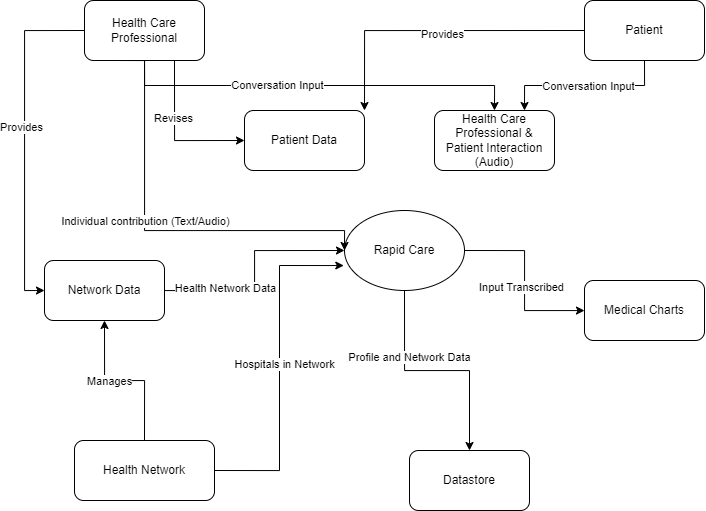
\includegraphics[width=0.8\textwidth]{System_Context.png}
  \caption{This is the System Context diagram for this scenario.}
  % \label{fig:Use-Case Diagram}
\end{figure}

\begin{itemize}
  \item \textbf{Inputs:}
  \begin{itemize}
    \item Audio from healthcare professionals and patient interaction.
    \item Keyboard input.
  \end{itemize}
  \item \textbf{Outputs:}
  \begin{itemize}
    \item Transcription of audio into text.
    \item Classification of text into clinical notes.
    \item Diagnosis and medication suggestions.
  \end{itemize}
  \item \textbf{User Responsibilities:}
  \begin{itemize}
    \item Record audio.
    \item Amend or delete documentation as needed.
    \item Maintain existing data, and journey tracks.
  \end{itemize}
  \item \textbf{System Responsibilities:}
  \begin{itemize}
    \item Accurately transcribe audio into text and classify it.
    \item Accurate mapping of patient journey in application.
  \end{itemize}

\item{\textbf{Expected Benefits:}}

\begin{itemize}
  \item Reduced documentation overhead time
  \item Increased patient throughput
  \item Improved patient care
  \item Increased doctor and healthcare professional satisfaction
\end{itemize}
\end{itemize}
Much like how copilot is a tool for programmers, the aim is to create a tool for healthcare professionals to help with documentation such that the number of patient processed per day can be increased, and the focus of doctors and nurses can be shifted from documentation to patient care.


\subsection{Work Partitioning}
\lips
% not completed

\subsection{Specifying a Business Use Case (BUC)}

\textbf{Main Usage Scenario: Documenting a Patient Consultation}

\begin{itemize}
  \item\textbf{Use Case:} UC2, UC3
  \item\textbf{Primary Actor:} Healthcare professional (such as a medical doctor or a nurse)
  \item\textbf{Precondition:} The user has been successfully authenticated, logged into the system and has patient's profile is created. The basic information such as name, contact information, and history is prefilled.
  \item\textbf{Trigger:} The user will initiate dictation.
  \item\textbf{Main Success Scenario:}
  \begin{itemize}
    \item The user will initiate dictation.
    \item The system will convert audio to text in real-time.
    \item The user will press stop button.
    \item The user reviews the transcribed notes. 
    \item The system has accurately transcribed the audio to text without any inaccuracies.
    \item The user selects the submit button after review. 
  \end{itemize}
  \item\textbf{Secondary Success Scenario:}
  \begin{itemize}
    \item The system has produced some inaccuracies in the transcribed text.
    \begin{itemize}
      \item The user selects the edit button.
      \item The system prompts user to edit the text.
      \item The user manually edits the transcribed text.
    \end{itemize} 
  \end{itemize}
  \item\textbf{Success Postcondition:}
  \begin{itemize}
    \item The notes are successfully saved in patient database and changes are reflected in the user interface.
  \end{itemize}
\end{itemize}

\section{Business Data Model and Data Dictionary}
\subsection{Business Data Model}
\lips
\subsection{Data Dictionary}
\lips

\section{The Scope of the Product}
\subsection{Product Boundary}
The scope of this project can be be split into the following:

\begin{itemize}
  \item \textbf{Out of Scope:}
  \begin{itemize}
    \item The system will not be responsible for patient scheduling, billing, or other administrative tasks.
    \item The system will not include development of any hardware components. All needed peripherals will be assumed as apart of the runtime environment.
  \end{itemize}
  \item \textbf{Typical Values of Input}
  \begin{itemize}
    \item The primary input mode will be audio, allowing for transcription and segmentation of conversations.
    \item The other input is typing through a keyboard to amend or edit any documentation.
    \item Standard office environment is expected, with standard computer equipment (i.e. mice, keyboards, internet).
  \end{itemize}
\end{itemize}

\subsection{Product Use Case Table}
% not completed

\subsection{Individual Product Use Cases (PUC's)}

\begin{itemize}
  \item\textbf{UC1 Login:}
  \begin{itemize}
    \item The user accesses the system using an internet browser.
    \item The user enters valid credentials on the log in page.
    \item The user selects the login button.
    \item The user lands on the default dashboard.
  \end{itemize}
  \item\textbf{UC2 Recording Clinical Notes:}
  \begin{itemize}
    \item The user accesses patient's record.
    \item The user initiates dictation.
    \item The user dictates the notes and hit the stop button.
    \item The user reviews the transcribed text.
    \item The user selects the submit button.
  \end{itemize}
  \item\textbf{UC3 Diagnostic Suggestions:}
  \begin{itemize}
    \item The user submits the transcribed text.
    \item The user reviews the potential diagnostic suggestions.
    \item The user accepts or rejects suggestions.
  \end{itemize}
  \item\textbf{UC4 Create Patient Profile:}
  \begin{itemize}
    \item The user log into the system.
    \item The user selects the 'create a new record' button.
    \item The user provide input for the required fields.    
    \item The user selects the submit button.
  \end{itemize}
\end{itemize}

\begin{figure}[H]
  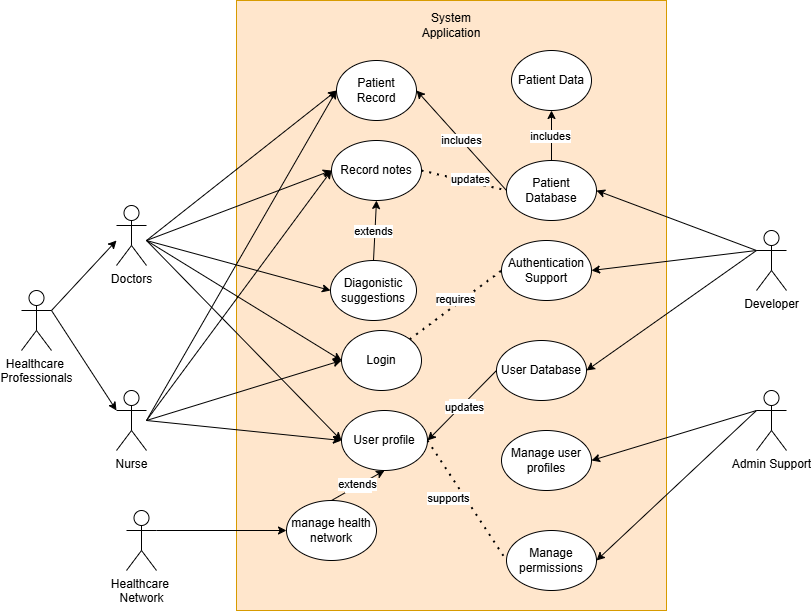
\includegraphics[width=0.8\textwidth]{use-case.drawio.png}
  \caption{This is the use-case diagram for this scenario.}
  \label{fig:Use-Case Diagram}
\end{figure}


\section{Functional Requirements}
\subsection{Functional Requirements}


\noindent \begin{itemize}

  \item [FR\refstepcounter{reqnum}\thereqnum \label{FR_addHealthNetwork}:] 
  
  \textbf{Requirement:} The system should allow a healthcare network to be onboarded to the system.
  
  \textbf{Rationale:} Rapid care is an organizational tool, where networks can register their various hospitals, and in turn add the corresponding health care professionals. When the networks want to register, the app needs to be able to add the network to the database along with the relevant staff profiles etc.
  
  \textbf{Fit Criterion:} The network data and profiles are fully added to the database. This could be verified by returning the valid entries from the patient database.
  
  \textbf{Dependencies:} N/A
  
  \textbf{Monitored and Controlled Variables:} N/A
  
  \textbf{Performance Requirements:} 
  \begin{itemize}
    \item The system should update the entries with the latency of 1 second.
    \item After user input is taken the system only adds valid entries to the database and prevents any data leaks.
  \end{itemize}
  
  \textbf{Hardware Requirements:} 
  \begin{itemize}
    \item Workstations and other peripherals to access the system.
  \end{itemize}
  
  \textbf{Software Requirements:} 
  \begin{itemize}
    \item Database management system to store health network data.
    \item Internet browser to access the application.
  \end{itemize}
  
  \textbf{Normal Behavior:} 
  \begin{itemize}
    \item All input data is validated as being entered into the system.
    \item Once all required fields are completed the user selects the submits the information and the network is added successfully to the system.
    \item The process should have a low turnover time such that health networks will not have to spend a long time waiting to use the system.
  \end{itemize}
  
  \textbf{Undesired Event Handling:} 
  \begin{itemize}
    \item The user may enter invalid input data. The system should display appropriate error messages. 
    \item The system should have constraints to restrict the user from submitting, unless all required fields are completed and have valid input data. 
    \item When the database is overloaded with requests, appropriate error messages should be delayed. 
    \item The updates will be queued to prevent this in the future, data resources will be scaled just so that the calls are faster.
  \end{itemize}
  
  
  \item[FR\refstepcounter{reqnum}\thereqnum \label{FR_removeHealthNetwork}:]  
  
  \textbf{Requirement:} The system should allow health network to remove itself from the system.
  
  \textbf{Rationale:} 
  When health networks close and want to pivot to another documentation tool their data and profiles must be deleted. Therefore, there is a requirement for functionality that allows organizations to deregister and have their data deleted.
  
  \textbf{Fit Criterion:} 
  The network data and profiles are fully deleted from the database. This could be verified by returning the valid entries from the patient database.
  
  \textbf{Dependencies:} FR\ref{FR_addHealthNetwork} 
  
  \textbf{Monitored and Controlled Variables:} N/A
  
  \textbf{Performance Requirements:} 
  \begin{itemize}
    \item The removal process must be easy to complete with a latency of 1 second. 
    \item The system should be able to identify the correct record to delete. 
    \item The system should delete the correct record without affecting the rest of the database. 
  \end{itemize}
  
  \textbf{Hardware Requirements:} 
  \begin{itemize}
    \item Workstations and other peripherals to access the system.
  \end{itemize}
  
  \textbf{Software Requirements:}
  \begin{itemize}
    \item Access to health network database.
    \item Internet browser to access the application.
  \end{itemize}
  
  \textbf{Normal Behavior:}
  \begin{itemize}
    \item Network is successfully removed from database with low turnover time such that health networks will not have to spend a long time waiting for their data to be deleted.
  \end{itemize}
  
  \textbf{Undesired Event Handling:}
  \begin{itemize}
    \item If the system fails to delete the health network due to a system error, the system should display an appropriate error message. 
    \item When the database is overloaded with requests, the operation to delete all the hospital data will be queued as the next action in line.
  \end{itemize}
  
  
  \item[FR\refstepcounter{reqnum}\thereqnum \label{FR_UpdateHealthNetwork}:]
  
  \textbf{Requirement:} The healthcare network should be able to update its organizational and hospital information.
  
  \textbf{Rationale:} The healthcare network will update its own organizational changes. This will include creating and maintaining the staff present as well as the hospitals in the network.
  
  \textbf{Fit Criterion:} The healthcare network data will be up to date with its current state (i.e. number of hospitals, staff etc.), the data's recency will depend on the networks need. 
  
  \textbf{Dependencies:} FR\ref{FR_addHealthNetwork}
  
  \textbf{Monitored and Controlled Variables:} N/A
  
  \textbf{Performance Requirements:} 
  \begin{itemize}
    \item The updating process of healthcare networks should be quick and easy so that healthcare professionals remain up to date with the facility information, operational data, healthcare professional data, and patient data.
    \item Under a standard load the request should be fulfilled within 1 second.
  \end{itemize}
  
  \textbf{Hardware Requirements:} 
  \begin{itemize}
    \item Workstations and other peripherals to access the system.
  \end{itemize}
  
  \textbf{Software Requirements:} 
  \begin{itemize}
    \item Internet browser to access the application.
  \end{itemize}
  
  \textbf{Normal Behavior:}
  \begin{itemize}
    \item Network is updated in the database without any leaks or latency.
    \item Normal behavior will be seen as updated reflected on the front-end and backend of the system.
  \end{itemize} 
  
  \textbf{Undesired Event Handling:} 
  \begin{itemize}
    \item When the health network data is being updated and the database is overloaded with requests, then updates will be queued.
  \end{itemize}
  
  \item[FR\refstepcounter{reqnum}\thereqnum \label{FR_AddHealthProfessional}:]
  
  \textbf{Requirement:} The system should allow healthcare network administrators to add healthcare professionals to the system.
  
  \textbf{Rationale:} When new healthcare professionals join the healthcare network, their information is to be added to the system for authentication purposes. This will include adding a list of hospital staff members to the network.
  
  \textbf{Fit Criterion:} The healthcare professional's data will be up to date in the system so that they can get authenticated without any delay. 
  
  \textbf{Dependencies:} N/A 
  
  \textbf{Monitored and Controlled Variables:} N/A
  
  \textbf{Performance Requirements:} 
  \begin{itemize}
    \item The addition process should be quick and easy to ensure that all professionals can access the database without any interruptions, with a minimum uptime of 99.5\%.
  \end{itemize}
  
  \textbf{Hardware Requirements:} 
  \begin{itemize}
    \item Workstations and other peripherals to access the system.
  \end{itemize}
  
  \textbf{Software Requirements:} 
  \begin{itemize}
    \item Internet browser to access the database.
  \end{itemize}
  
  \textbf{Normal Behavior:}
  \begin{itemize}
    \item Data is added to the database without any leaks or latency. Normal behavior will be seen as updated are reflected in database and UI of the system.
  \end{itemize} 
  
  \textbf{Undesired Event Handling:}
  \begin{itemize}
    \item When the healthcare professional's data is being added and the database is overloaded with requests, then updates will be queued.
  \end{itemize} 
  
  \item[FR\refstepcounter{reqnum}\thereqnum \label{FR_RemoveHealthProfessionals}:] 
  
  \textbf{Requirement:} The system should allow healthcare network administrators to remove healthcare professionals from the system. 
  
  \textbf{Rationale:} Sometimes a healthcare professional decides to change the area of service or leaves the organization and retires. Therefore, there is a need for functionality that allows to remove them from the system.
  
  \textbf{Fit Criterion:} The healthcare professional is successfully removed from the system, this will be verified by the fact that they are not present in the databases. 
  
  \textbf{Dependencies:} FR\ref{FR_AddHealthProfessional}
  
  \textbf{Monitored and Controlled Variables:} N/A
  
  \textbf{Performance Requirements:}
  \begin{itemize}
    \item The deleting process must be easy to complete with a low turnover time such that health networks will not have to spend a long time waiting for their data to be deleted.
  \end{itemize} 
  
  \textbf{Hardware Requirements:}
  \begin{itemize}
    \item Workstations and other peripherals to access the system.
  \end{itemize} 
  
  \textbf{Software Requirements:}
  \begin{itemize}
    \item Internet browser to access the database.
  \end{itemize} 
  
  \textbf{Normal Behavior:}
  \begin{itemize}
    \item Data is removed to the database without any leaks or latency. Normal behavior will be seen as updated are reflected on the frontend and backend of the system.
  \end{itemize} 
  
  \textbf{Undesired Event Handling:}
  \begin{itemize}
    \item When the healthcare professional's data is being removed and the database is overloaded with requests, then updates will be queued.
  \end{itemize} 
  
  \item[FR\refstepcounter{reqnum}\thereqnum \label{FR_UpdateHealthProfessionals}:]
  
  \textbf{Requirement:} The system should allow healthcare network administrators to update healthcare professional's data in the system.
  
  \textbf{Rationale:} Sometimes healthcare professionals receive promotions or other changes in their roles which require updating the information in their profiles. Therefore, it is essential for functionality that allows to edit the data in case there are inaccuracies.  
  
  \textbf{Fit Criterion:} The healthcare professional's data will be up to date in its current state (i.e. role of each healthcare professional and the organization they work in etc). 
  
  \textbf{Dependencies:} FR\ref{FR_AddHealthProfessional}
  
  \textbf{Monitored and Controlled Variables:} N/A
  
  \textbf{Performance Requirements:} 
  \begin{itemize}
    \item The changes should be reflected in real time on the UI.
    \item The changes should be stored successfully in the database.
  \end{itemize} 
  
  \textbf{Hardware Requirements:}
  \begin{itemize}
    \item Workstations and other peripherals to access the system.
  \end{itemize} 
  
  \textbf{Software Requirements:}
  \begin{itemize}
    \item Internet browser to access the database.
  \end{itemize} 
  
  \textbf{Normal Behavior:}
  \begin{itemize}
    \item Data is updated in the database without any leaks or latency. Normal behavior will be seen as updated are reflected on the front-end and backend of the system.
  \end{itemize} 
  
  \textbf{Undesired Event Handling:}
  \begin{itemize}
    \item When the healthcare professional's data is being updated and the database is overloaded with requests, then updates will be queued.
  \end{itemize} 
  
  \item[FR\refstepcounter{reqnum}\thereqnum \label{FR_login}:]
  
  \textbf{Requirement:} The system should allow the authorized user to successfully log in to the system.
  
  \textbf{Rationale:} Doctors and other medical professionals should be able to log into the system to create patients, update, and delete patient records and access their medical records. The system should also authenticate the user to avoid unauthorized access to the data.
  
  \textbf{Fit Criterion:} The system only authenticates the authorized users to log into the system and has 100\% accuracy. 
  
  \textbf{Dependencies:} FR\ref{FR_AddHealthProfessional}, FR\ref{NFR_Security}
  
  \textbf{Monitored and Controlled Variables:} number of failed login attempts
  
  \textbf{Performance Requirements:} 
  \begin{itemize}
    \item The system successfully redirects users to correct system state based on authentication.
  \end{itemize}
  
  \textbf{Hardware Requirements:} 
  \begin{itemize}
    \item Workstations and other peripherals to access the system.
  \end{itemize}
  
  \textbf{Software Requirements:} 
  \begin{itemize}
    \item Authentication protocols and encryption for security. 
    \item Internet browser to access the system.
  \end{itemize}
  
  \textbf{Normal Behavior:} 
  \begin{itemize}
    \item The user is able to successfully login upon providing valid credentials and is redirected to the appropriate dashboard based on their role.
  \end{itemize}
  
  \textbf{Undesired Event Handling:}
  \begin{itemize}
    \item If a user provides invalid credentials, the system will display an error message and redirect the user to sign in page.
    \item After three failed login attempts, the user account will be locked, and the user will have to contact the support team to regain access.
  \end{itemize}
   
  
  \item[FR\refstepcounter{reqnum}\thereqnum \label{FR_createRecord}:]
  
  \textbf{Requirement:} The user should be able to create a new patient record. 
  
  \textbf{Rationale:} The patient data and medical history must be stored in a secure manner. Therefore, medical staff should be able to create a new patient record to store all the relevant information. 
  
  \textbf{Fit Criterion:} The record is created and added to the patient database. This could be verified by returning the valid entries from the patient database.
  
  \textbf{Dependencies:} FR\ref{FR_login}
  
  \textbf{Monitored and Controlled Variables:} field validation
  
  \textbf{Performance Requirements:} 
  \begin{itemize}
    \item The system should update the patient database with the latency of 1 second. 
    \item The system only adds valid entries to the database.
    \item The system prevents any data leaks.
  \end{itemize}
  
  \textbf{Hardware Requirements:} 
  \begin{itemize}
    \item Workstations and other peripherals to access the system.
  \end{itemize}
  
  \textbf{Software Requirements:} 
  \begin{itemize}
    \item Database management system to store patient information.
    \item Internet browser to access the system.
  \end{itemize}
  
  \textbf{Normal Behavior:} 
  \begin{itemize}
    \item All input data is validated as it is entered using field level validation. 
    \item Once all required fields are completed the user selects the submit button, a new patient record is successfully created and stored.
  \end{itemize}
  
  \textbf{Undesired Event Handling:} 
  \begin{itemize}
    \item The user may enter invalid input data. The system should display appropriate error messages. 
    \item The system should have constraints to restrict the user from submitting, unless all required fields are completed and have valid input data. 
    \item If the system fails to save the record due to a system error, the system should display an appropriate error message. 
  \end{itemize}
  
  
  \item[FR\refstepcounter{reqnum}\thereqnum \label{FR_deleteRecord}:]
  
  \textbf{Requirement:} The user should be able to delete an existing patient record from the system.
  
  \textbf{Rationale:} There can be instances where medical professionals need to delete a certain patient record, for example inaccurate entries, duplicate records etc. Therefore, the system should allow authorized users to remove patient records.
  
  \textbf{Fit Criterion:} The record is successfully removed from the patient database. This could be verified by returning the valid entries from the patient database.
  
  \textbf{Dependencies:} FR\ref{FR_login}, FR\ref{FR_createRecord}
  
  \textbf{Monitored and Controlled Variables:} N/A
  
  \textbf{Performance Requirements:} 
  \begin{itemize}
    \item The deletion process must be easy to complete with a latency of 1 second. 
    \item The system should be able to identify the correct record to delete. 
    \item The system should delete the correct record without affecting the rest of the database. 
  \end{itemize}
  
  \textbf{Hardware Requirements:} 
  \begin{itemize}
    \item Workstations and other peripherals to access the system.
  \end{itemize}
  
  \textbf{Software Requirements:} 
  \begin{itemize}
    \item Access to patient record database.
    \item Role based access control system to manage user permissions.
    \item Internet browser to access the system.
  \end{itemize}
  
  \textbf{Normal Behavior:} 
  \begin{itemize}
    \item The user selects the delete button and confirms the deletion. The patient record is successfully removed from the database and no longer appears on the system.
  \end{itemize}
  
  \textbf{Undesired Event Handling:} 
  \begin{itemize}
    \item If the user does not have permission to delete the record, the system should show an appropriate error message.
    \item If the system fails to delete the record due to a system error, the system should display an appropriate error message. 
  \end{itemize}
  
  
  
  \item[FR\refstepcounter{reqnum}\thereqnum \label{FR_updateRecordtyping}:]
  
  \textbf{Requirement:} : The system should allow the user to update the patient records manually by typing.
  
  \textbf{Rationale:} Medical professionals frequently need to update patient information, such as changes in diagnosis, medication, or medical history. The healthcare professional may want to add some information manually. Moreover, if healthcare professionals use the dictation tool, they still should be allowed to edit the auto filled transcribed data in case there are inaccuracies.
  
  \textbf{Fit Criterion:} The system should update the current state and patient database with the input information.
  
  \textbf{Dependencies:} FR\ref{FR_login}, FR\ref{FR_createRecord}
  
  \textbf{Monitored and Controlled Variables:} N/A
  
  \textbf{Performance Requirements:} 
  \begin{itemize}
    \item The changes should be reflected in real time on the user interface.
    \item The changes should be stored successfully in the database.
  \end{itemize}
  
  \textbf{Hardware Requirements:} 
  \begin{itemize}
    \item Workstations and other peripherals to access the system.
  \end{itemize}
  
  \textbf{Software Requirements:} 
  \begin{itemize}
    \item Access to patient record database.
    \item Internet browser to access the system. 
  \end{itemize}
  
  \textbf{Normal Behavior:} 
  \begin{itemize}
    \item The user edits the selected field and enters new information. 
    \item The system successfully updates the changes in database and reflect changes on the user interface. 
  \end{itemize}
  
  \textbf{Undesired Event Handling:}
  \begin{itemize}
    \item If an unauthorized user tries to update a record, the system displays appropriate error messages. 
    \item If the system fails to update the record due to a system error, the system should display an appropriate error message. 
  \end{itemize}
  
  \item[FR\refstepcounter{reqnum}\thereqnum \label{FR_DictationRecording}:]
  
  \textbf{Requirement:} The system should allow healthcare workers to update patient records using dictation. 
      
  \textbf{Rationale:} This will reduce the workload on the healthcare workers, while also efficiently reducing the time spent on documentation. 
      
  \textbf{Fit Criterion:} The system should use voice dictation to document medical reports with a minimum of 90\% accuracy. 
      
  \textbf{Dependencies:} FR\ref{FR_login}, FR\ref{FR_createRecord} 
      
  \textbf{Monitored Variables:} Accuracy
      
  \textbf{Performance:} 
    \begin{itemize}
        \item System should transcribe speech in real time and segment it into the right fields onto the record with a minimum of 90\% accuracy.
    \end{itemize}
      
  \textbf{Hardware Requirements:}
    \begin{itemize}
        \item Workstations to access the system and a microphone which can record the voice in the system. 
    \end{itemize}
      
  \textbf{Software Requirements:}
    \begin{itemize}
        \item An audio transcription service to transcribe audio to text 
        \item Access to patient record database. 
        \item Internet browser to access the system.  
    \end{itemize}
      
  \textbf{Normal Use:} 
  \begin{itemize}
    \item The system records the provider's voice and updates the patient file with the transcribed text.
  \end{itemize}
      
  \textbf{Undesired Event Handling:} 
  \begin{itemize}
    \item If the recording or transcription fails, the system should notify the user and offer manual review.
  \end{itemize}
  
  
  \item[FR\refstepcounter{reqnum}\thereqnum \label{FR_DiagnosticSuggestions}:]
  
  \textbf{Requirement:} The system should analyze transcribed text and provide diagnostic suggestions based on the input.
      
  \textbf{Rationale:} This alerts the healthcare professionals about the possible diagnostics and helps them to diagnose the patients quicker based on suggested options.
      
  \textbf{Fit Criterion:} The system must suggest diagnoses within 5 seconds after transcript is provided, with 85\% accuracy based on known patient's medical record.
      
  \textbf{Dependencies:} FR\ref{FR_DictationRecording}
      
  \textbf{Monitored Variables:} Suggested diagnostic accuracy, time to generate suggestions 
    
  \textbf{Performance:}
    \begin{itemize}
      \item Suggestions must be provided within 5 seconds of transcript completion. 
      \item Suggestions should match known diagnoses with 85\% accuracy. 
    \end{itemize}
      
  \textbf{Hardware Requirements:}
    \begin{itemize}
      \item Workstations and other peripherals to access the system. 
    \end{itemize}
      
  \textbf{Software Requirements:}
    \begin{itemize}
      \item Access to patient record database. 
      \item Internet browser to access the system.  
      \item Service engine that generates diagnostic suggestions. 
    \end{itemize}
      
  \textbf{Normal Use:} 
    \begin{itemize}
      \item The system analyzes the transcribed conversation and suggests possible diagnoses based on a patient's medical record. 
    \end{itemize}
      
  \textbf{Undesired Event Handling:} 
    \begin{itemize}
      \item If the system can't suggest a diagnosis, it should notify the user and offer a manual search option. 
    \end{itemize}
  
  
  \item[FR\refstepcounter{reqnum}\thereqnum \label{FR_medicalSuggestions}:] 
  
  \textbf{Requirement:} The system should provide a list of frequently used medicines based on accepted diagnosis.
  
  \textbf{Rationale:} As the patients' medical records and data is being added into the charts, having a model that can provide a preliminary set of diagnosis such that documentation time can be saved. This supplementary tool will provide auto-completion analogous to what auto-completion tools programmers use.
  
  \textbf{Fit Criterion:} Auto-completion suggestions regarding diagnoses and medicine are applicable 85+\% of the time. The model will be measured through cross validation techniques.
   
  \textbf{Dependencies:} FR\ref{FR_DictationRecording}, FR\ref{FR_DiagnosticSuggestions}
  
  \textbf{Monitored and Controlled Variables:} accuracy
  
  \textbf{Performance Requirements:}
  \begin{itemize}
    \item The autocompletion is accurate, such that it is correct 85+\% of the time. 
  \end{itemize}
  
  \textbf{Hardware Requirements:} 
  Workstations and other peripherals to access the system.
  
  \textbf{Software Requirements:}
  \begin{itemize}
    \item Access to patient record database.
    \item Internet browser to access the system. 
  \end{itemize}
  
  \textbf{Normal Behavior:}
  \begin{itemize}
    \item A list of medicine suggestion is provided almost instantly analogous to an auto-complete feature based on the selected diagnosis.
  \end{itemize}
  
  \textbf{Undesired Event Handling:}
  \begin{itemize}
    \item In case no medicine suggestions are provided the doctor can manually add a prescription.
  \end{itemize}
  
  \item[FR\refstepcounter{reqnum}\thereqnum \label{FR_transferPatient}:] 
  \textbf{Requirement:} The system should be able to transfer patient documentation to another provider. 
  
  \textbf{Rationale:} If the patient goes to a hospital in another health network, perhaps the medical history is to be shared. This functionality will allow the request and transfer of files.
  
  \textbf{Fit Criterion:} Transfer over the files in a short time, the transfer protocol is secure, and data is not leaked.
  
  \textbf{Dependencies:} FR\ref{FR_createRecord}
  
  \textbf{Monitored and Controlled Variables:} N/A
  
  \textbf{Performance Requirements:}
  \begin{itemize}
    \item The system should transfer data with a latency of less than 1 seconds.
  \end{itemize}
  
  \textbf{Hardware Requirements:} 
  \begin{itemize}
    \item Workstations and other peripherals to access the system.
  \end{itemize}
  
  \textbf{Software Requirements:}
  Access to patient record database.
  \begin{itemize}
    \item Internet browser to access the system. 
  \end{itemize}
  
  \textbf{Normal Behavior:}
  \begin{enumerate}
    \item A patient file is requested
    \item The request is approved then the files are transferred.
  \end{enumerate}
  -
  \textbf{Undesired Event Handling:}
  \begin{enumerate}
    \item A patient file is requested 
    \item The request for the file is denied. 
    \item A detailed request is submitted for approval to provide further information that may have been missing.
  \end{enumerate}
  \end{itemize}


  \section{Look and Feel Requirements} \label{NFR_LookAndFeel}
  \subsection{Appearance Requirements}
  The user interface (UI) of the system should have a clean and modern design that prioritizes simplicity and ease of navigation. The UI should be visually appealing and intuitive, ensuring that users can quickly locate core functions without additional guidance. The design should reduce excess noise and make the interface as simple as possible, allowing healthcare professionals to focus on patient care rather than managing the system.
  
  \subsection{Style Requirements}
  The system should adhere to a consistent style guide, including color schemes, typography, and layout. The style should be professional and align with healthcare standards, ensuring that the system is easy to use for healthcare professionals of all skill levels. The UI should be designed to be accessible and inclusive, accommodating users with varying technical expertise and diverse educational backgrounds.
  
  \section{Usability Requirements} \label{NFR_Usability}
  \subsection{Ease of Use Requirements}
  The system should be highly intuitive, ensuring that healthcare workers can effectively use the system after a brief 30-minute training session. The system should allow users to perform key functions such as logging in, accessing patient records, adding entries, and generating reports without assistance. The majority of users should be able to locate core functions without additional guidance.
  
  \subsection{Personalization Requirements}
  The system allows for limited personalization, where hospitals can add and manage their employees, and healthcare professionals can create and update patient records. Each hospital can customize the system by adding their staff members, while healthcare professionals can personalize the system by creating new patient profiles and adding relevant medical files. This ensures that the system is tailored to the specific needs of each hospital and healthcare professional, while maintaining a consistent and user-friendly interface for all users.
  
  \subsection{Learning Requirements}
  The system should be designed to minimize the learning curve for new users. Healthcare professionals should be able to learn and use the system quickly, with minimal training. The system should provide clear instructions and guidance for users to navigate and perform tasks efficiently.
  
  \subsection{Understandability and Politeness Requirements}
  The system should provide clear and concise error messages that guide users to recover from errors. The system should be polite and respectful in its interactions with users, ensuring that users feel confident and supported while using the system.
  
  \subsection{Accessibility Requirements}
  The system should meet established accessibility standards to ensure usability for all healthcare staff, including those with disabilities. The UI should be designed for ease of navigation, incorporating various accessibility features such as step-by-step instructions and support for assistive technologies.
  
  \section{Performance Requirements} \label{NFR_Performance}
  \subsection{Speed and Latency Requirements}
  The system should provide responsive voice-to-text conversion, with real-time transcription displayed within a 2-second delay. The system should maintain high processing throughput during peak operational loads, ensuring that users can complete tasks quickly and efficiently.
  
  \subsection{Safety-Critical Requirements}
  The system should ensure the accuracy and reliability of transcribed medical data. Misinterpretation of words could lead to inaccurate records and wrong diagnoses, so the system must provide accurate transcriptions with a minimum accuracy of 85\%.
  
  \subsection{Accuracy Requirements}
  The system should provide accurate transcriptions of voice input, with a minimum accuracy of 85\%. The system should also provide accurate diagnostic and medication suggestions based on the transcribed data, with a confidence score exceeding 85\%.
  
  \subsection{Robustness Requirements}
  The system should maintain stability and uptime of 99.9\% or above during operational hours. The system should handle unexpected or invalid inputs gracefully, providing appropriate error messages and guiding users to recover from errors.
  
  \subsection{Capacity Requirements}
  The system should be capable of handling an increasing number of concurrent users without degradation in performance. The system should scale horizontally to support concurrent users while maintaining consistent response times.
  
  \subsection{Scalability Requirements}
  The system should be scalable to accommodate future growth and additional features. The system should be designed to integrate with existing hospital environments and support future enhancements without significant rework.
  
  \subsection{Longevity Requirements}
  The system should be designed for long-term use, with regular updates and maintenance to ensure continued reliability and performance. The system should be adaptable to changes in healthcare regulations and technological advancements.
  
  \section{Operational Requirements} \label{NFR_Operational}
  \subsection{Expected Physical Environment}
  The system is expected to operate in a standard office environment with standard computer equipment, such as monitors, keyboards, and internet access. The system should be compatible with typical clinic noise levels and other environmental factors.
  
  \subsection{Wider Environment Requirements}
  The system should comply with healthcare regulations and data protection standards, ensuring the confidentiality and security of patient data. The system should be designed to operate in a cloud-based environment.
  
  \subsection{Requirements for Interfacing with Adjacent Systems}
  The system should integrate seamlessly with existing hospital systems, such as Electronic Health Record (EHR) systems. The system should support data exchange and interoperability with other healthcare systems to ensure a smooth workflow.
  
  \subsection{Productization Requirements}
  The system should be designed for easy deployment and maintenance, with clear documentation and support for regular updates. The system should be packaged and distributed in a way that allows for easy installation and configuration.
  
  \subsection{Release Requirements}
  The system should undergo rigorous testing and validation before release to ensure that it meets all functional and non-functional requirements. The system should be released with comprehensive user documentation and support materials.
  
  \section{Maintainability Requirements} \label{NFR_Maintainability}
  \subsection{Maintenance Requirements}
  The system should undergo regular updates for bug fixes and feature enhancements, ensuring minimal disruption to users. The system should be designed to be modular and maintainable, allowing for easy updates and modifications.
  
  \subsection{Supportability Requirements}
  The system should provide clear documentation and support resources for users and administrators. The system should include logging and monitoring tools to assist in troubleshooting and resolving issues.
  
  \subsection{Adaptability Requirements}
  The system should be adaptable to changes in healthcare regulations, technological advancements, and user needs. The system should be designed to support future enhancements and integrations without significant rework.
  
  \section{Security Requirements} \label{NFR_Security}
  \subsection{Access Requirements}
  The system should provide secure user authentication methods to ensure that only authorized personnel can access sensitive patient information. Unauthorized access attempts should be blocked and logged, with notifications sent to the security team.
  
  \subsection{Integrity Requirements}
  The system should ensure the integrity of patient data by validating input data and preventing unauthorized modifications. The system should log all actions and provide audit trails for review by the security team.
  
  \subsection{Privacy Requirements}
  The system should comply with data protection regulations, such as PIPEDA, to ensure the privacy and confidentiality of patient data. The system should handle patient data securely and prevent unauthorized access or data breaches.
  
  \subsection{Audit Requirements}
  The system should provide logging and audit trails for all actions, including access attempts, data modifications, and system updates. The system should allow administrators to review logs and audit trails to ensure compliance with security policies.
  
  \subsection{Immunity Requirements}
  The system should be designed to resist common security threats, such as unauthorized access, data breaches, and denial-of-service attacks. The system should include security measures to protect against these threats and ensure the continued operation of the system.
  
  \section{Cultural Requirements} \label{NFR_Cultural}
  \subsection{Cultural Sensitivity Requirements}
  The system should ensure that all content, including transcribed text and generated reports, is culturally sensitive and free from inappropriate language. The system must avoid any offensive or culturally insensitive content in its output, ensuring that it is professional and respectful in all interactions with users.
  
  \section{Legal Requirements}  \label{NFR_Legal}
  \subsection{Compliance Requirements}
  The system should comply with all relevant healthcare data protection regulations, such as PIPEDA. The system should ensure that patient data is handled securely and in compliance with legal requirements.
  
  \subsection{Standards Compliance Requirements}
  The system should adhere to industry standards for software development, data security, and healthcare documentation. The system should be designed to meet or exceed these standards, ensuring that it is reliable and secure.


\section{Open Issues}
\lips

\section{Off-the-Shelf Solutions}
\subsection{Ready-Made Products}
\lips
\subsection{Reusable Components}
\lips
\subsection{Products That Can Be Copied}
\lips

\section{New Problems}
\subsection{Effects on the Current Environment}
\lips
\subsection{Effects on the Installed Systems}
\lips
\subsection{Potential User Problems}
\lips
\subsection{Limitations in the Anticipated Implementation Environment That May
Inhibit the New Product}
\lips
\subsection{Follow-Up Problems}
\lips

\section{Tasks}
\subsection{Project Planning}


\section{Phase-In Plan}

All requirements with High priority must be implemented prior to the Revision 0 demonstration as they represent the core functionality of our system.\\
FR\ref{FR_AddHealthProfessional}\\
FR\ref{FR_login}\\
FR\ref{FR_createRecord}\\
FR\ref{FR_deleteRecord}\\
FR\ref{FR_updateRecordtyping}\\ 
FR\ref{FR_DictationRecording}\\

All requirements with Medium priority will be implemented before the Revision 1 demonstration.\\
FR\ref{FR_addHealthNetwork}\\
FR\ref{FR_DiagnosticSuggestions}\\
FR\ref{FR_medicalSuggestions}\\

All requirements with Low priority will be added after all High and Medium requirements are implemented, time permitting.\\
FR\ref{FR_removeHealthNetwork}\\
FR\ref{FR_UpdateHealthNetwork}\\
FR\ref{FR_RemoveHealthProfessionals}\\
FR\ref{FR_UpdateHealthProfessionals}\\ 
FR\ref{FR_transferPatient}\\

\subsection{Planning of the Development Phases}
\lips

\section{Migration to the New Product}
\subsection{Requirements for Migration to the New Product}
\lips
\subsection{Data That Has to be Modified or Translated for the New System}
\lips

\section{Costs}
\lips
\section{User Documentation and Training}
\subsection{User Documentation Requirements}
\lips
\subsection{Training Requirements}
\lips

\section{Waiting Room}
\lips

\section{Ideas for Solution}
\lips


\newpage
    \begin{landscape}
      \section{Traceability Matrices and Graphs}
      \begin{table}[H]
      \begin{tabular}{|c|c|c|c|c|c|c|c|c|c|c|c|c|c|c|c|c|c|c|c|c|c|c|}
      \hline
      & \rotatebox{90}{FR\ref{FR_addHealthNetwork}} & \rotatebox{90}{FR\ref{FR_removeHealthNetwork}} & \rotatebox{90}{FR\ref{FR_UpdateHealthNetwork}} & \rotatebox{90}{FR\ref{FR_AddHealthProfessional}} & \rotatebox{90}{FR\ref{FR_RemoveHealthProfessionals}} & \rotatebox{90}{FR\ref{FR_UpdateHealthProfessionals}} & \rotatebox{90}{FR\ref{FR_login}} & \rotatebox{90}{FR\ref{FR_createRecord}} & \rotatebox{90}{FR\ref{FR_deleteRecord}} & \rotatebox{90}{FR\ref{FR_updateRecordtyping}} & \rotatebox{90}{FR\ref{FR_DictationRecording}} & \rotatebox{90}{FR\ref{FR_DiagnosticSuggestions}} & \rotatebox{90}{FR\ref{FR_medicalSuggestions}} & \rotatebox{90}{FR\ref{FR_transferPatient}} & \rotatebox{90}{NFR\ref{NFR_LookAndFeel}} & \rotatebox{90}{NFR\ref{NFR_Usability}} & \rotatebox{90}{NFR\ref{NFR_Performance}} & \rotatebox{90}{NFR\ref{NFR_Operational}} & \rotatebox{90}{NFR\ref{NFR_Maintainability}} & \rotatebox{90}{NFR\ref{NFR_Security}} & \rotatebox{90}{NFR\ref{NFR_Cultural}} & \rotatebox{90}{NFR\ref{NFR_Legal}} \\
      \hline
      FR\ref{FR_addHealthNetwork} & - & - & - & - & - & - & - & - & - & - & - & - & - & - & - & - & - & - & - & - & - & - \\ \hline
      FR\ref{FR_removeHealthNetwork} & X & - & - & - & - & - & - & - & - & - & - & - & - & - & - & - & - & - & - & - & - & - \\ \hline
      FR\ref{FR_UpdateHealthNetwork} & X & - & - & - & - & - & - & - & - & - & - & - & - & - & - & - & - & - & - & - & - & - \\ \hline
      FR\ref{FR_AddHealthProfessional} & - & - & - & - & - & - & - & - & - & - & - & - & - & - & - & - & - & - & - & - & - & - \\ \hline
      FR\ref{FR_RemoveHealthProfessionals} & - & - & - & X & - & - & - & - & - & - & - & - & - & - & - & - & - & - & - & - & - & - \\ \hline
      FR\ref{FR_UpdateHealthProfessionals} & - & - & - & X & - & - & - & - & - & - & - & - & - & - & - & - & - & - & - & - & - & - \\ \hline
      FR\ref{FR_login} & - & - & - & X & - & - & - & - & - & - & - & - & - & - & - & - & - & - & - & X & - & - \\ \hline
      FR\ref{FR_createRecord} & - & - & - & - & - & - & X & - & - & - & - & - & - & - & - & - & - & - & - & - & - & - \\ \hline
      FR\ref{FR_deleteRecord} & - & - & - & - & - & - & X & X & - & - & - & - & - & - & - & - & - & - & - & - & - & - \\ \hline
      FR\ref{FR_updateRecordtyping} & - & - & - & - & - & - & X & X & - & - & - & - & - & - & - & - & - & - & - & - & - & - \\ \hline
      FR\ref{FR_DictationRecording} & - & - & - & - & - & - & X & X & - & - & - & - & - & - & - & - & - & - & - & - & - & - \\ \hline
      FR\ref{FR_DiagnosticSuggestions} & - & - & - & - & - & - & - & - & - & - & X & - & - & - & - & - & - & - & - & - & - & - \\ \hline
      FR\ref{FR_medicalSuggestions} & - & - & - & - & - & - & - & - & - & - & X & X & - & - & - & - & - & - & - & - & - & - \\ \hline
      FR\ref{FR_transferPatient} & - & - & - & - & - & - & - & X & - & - & - & - & - & - & - & - & - & - & - & - & - & - \\ \hline
      NFR\ref{NFR_LookAndFeel} & - & - & - & - & - & - & - & - & - & - & - & - & - & - & - & - & - & - & - & - & - & - \\ \hline
      NFR\ref{NFR_Usability} & - & - & - & - & - & - & - & - & - & - & - & - & - & - & X & - & - & - & - & - & - & - \\ \hline
      NFR\ref{NFR_Performance} & - & - & - & - & - & - & - & - & - & - & X & - & - & - & - & - & - & X & - & - & - & - \\ \hline
      NFR\ref{NFR_Operational} & - & - & - & - & - & - & - & - & - & - & X & - & - & - & - & - & - & - & - & - & - & X \\ \hline
      NFR\ref{NFR_Maintainability} & - & - & - & - & - & - & - & - & - & - & - & - & - & - & - & - & - & - & - & - & - & - \\ \hline
      NFR\ref{NFR_Security} & - & - & - & - & - & - & - & - & - & - & - & - & - & - & - & - & - & - & - & - & - & - \\ \hline
      NFR\ref{NFR_Cultural} & - & - & - & - & - & - & - & - & - & - & - & - & - & - & - & - & - & - & - & - & - & - \\ \hline
      NFR\ref{NFR_Legal} & - & - & - & - & - & - & - & - & - & - & - & - & - & - & - & - & - & - & - & - & - & - \\ \hline
      \end{tabular}
      \caption{Traceability Matrix Showing the Connections Between Requirements}
      \label{Table:A_trace}
      \end{table}
    \end{landscape}


\section{Development Plan}
N/A


~\newpage

\section{References}
\begin{itemize}
  \item
  [1]N. Ireland, "Number of Ontarians without family doctor reaches 2.5 million, college says," CBC, Jul. 12, 2024. https://www.cbc.ca/news/canada/toronto/ontario-family-doctor-shortage-record-high-1.7261558
  \href{https://www.cbc.ca/news/canada/toronto/ontario-family-doctor-shortage-record-high-1.7261558}{Article on Doctor Shortage.}
  \item 
  [2]Ryan Patrick Jones, "Family doctor shortage affects every region and is getting worse, Ontario Medical Association says," CBC, Jan. 29, 2024.
  
  https://www.cbc.ca/news/canada/toronto/family-doctor-shortage-oma-1.7097935
  \href{https://www.cbc.ca/news/canada/toronto/family-doctor-shortage-oma-1.7097935}{Article on Doctor Shortage.}
  \item
  [3]"ICES | Association between waiting times and short term mortality and hospital admission after departure from the emergency department: population-based cohort study from Ontario, Canada," ICES, Jun. 14, 2023. https://www.ices.on.ca/publications/journal-articles/association-between-waiting-times-and-short-term-mortality-and-hospital-admission-after-departure-from-the-emergency-department-population-based-cohort-study-from-ontario-canada/ (accessed Oct. 12, 2024).
  \href{https://www.ices.on.ca/publications/journal-articles/association-between-waiting-times-and-short-term-mortality-and-hospital-admission-after-departure-from-the-emergency-department-population-based-cohort-study-from-ontario-canada/}{Article on ER patients leaving without being seen.}
\end{itemize}

\newpage{}
\section*{Appendix --- Reflection}

The information in this section will be used to evaluate the team members on the
graduate attribute of Lifelong Learning.  Please answer the following questions:

\begin{enumerate}
  \item What went well while writing this deliverable?
  
  This document has let us build more on the rough ideas we had brainstormed initially. While going through the outline of this document, we were able to provide the functional and non-functional requirements of the system. It also made us better understand the detailed procedure of automation using the use-case diagram. 

  \item What pain points did you experience during this deliverable, and how did
  you resolve them?

  There are obstacles in any team project that must be overcome for it to proceed successfully. To ensure seamless operations, we had to develop a strategy for contributions. We must plan a template that aligns with our project to make sure we have all the requirements for the system. We also needed to create a schedule to contribute to the template and review each other's work in the best way possible.
  
  \item How many of your requirements were inspired by speaking to your
  client(s) or their proxies (e.g. your peers, stakeholders, potential users)?

  The stakeholder didn't explicitly contribute to the requirements section of the project, however, the stakeholder did give us her insight on the working of the software and EMR apps in clinics and hospitals. This helped us to refine our usage scenario diagram and has been a great source of help in the progress of the project.

  \item Which of the courses you have taken, or are currently taking, will help
  your team to be successful with your capstone project.

  In terms of courses, we have taken our requirements course (SFWRENG 3RA3), system design course (SFWRENG 3A04), as well as our testing course (SFWRENG 3S03). These courses have helped us develop the requirement documents but also prepared us in the sense that we are able to look into the future to what the testing and design strategy should look like. These courses have played a pivotal role in our understanding and creation of our documents. 

  \item What knowledge and skills will the team collectively need to acquire to
  successfully complete this capstone project?  Examples of possible knowledge
  to acquire include domain specific knowledge from the domain of your
  application, or software engineering knowledge, mechatronics knowledge or
  computer science knowledge.  Skills may be related to technology, or writing,
  or presentation, or team management, etc.  You should look to identify at
  least one item for each team member.

  As different abilities are added to the overall development plan, the project progresses more quickly thanks to the diversified knowledge of the team members. Technical expertise in data processing and integration would be very beneficial for this capstone project. In addition, time management abilities are required to make sure that everyone is moving at the same rate and that they are informed about each other's work to prevent backlogs. Additionally, being able to work on backend programming with an understanding of different server-side technologies, like Python, Java, and React.js, will be helpful in creating a dynamic database that secures patient data. 

  \item For each of the knowledge areas and skills identified in the previous
  question, what are at least two approaches to acquiring the knowledge or
  mastering the skill?  Of the identified approaches, which will each team
  member pursue, and why did they make this choice?

  One can use a variety of resources to learn Java from Spring and Python from Flask to become effective in backend programming. With these resources, developers can gain practical experience by building web applications that offer them flexibility. Using LeetCode to practice coding skills is an additional strategy. This allows users to modify the difficulty of the problems and proceed with their solution. Moreover, setting goals and taking regular pauses between tasks might help with time management and allow one to work more effectively. It's critical that each member of the team grasp every talent for everyone to be moving at the same speed. This is because it's a fantastic chance to learn and implement it in practical situations. 

\end{enumerate}

\end{document}